% !TeX spellcheck = en_US
\chapter{Theory and methodology}%
As mentioned in previous sections, forming a virtual experiment platform 
is necessary for investigating the temperature estimation algorithm. So, a virtual 
experiment platform is developed based on Planks'law, then, a virtual multi-spectral 
pyrometer is applied to obtain the digital value (also called image). 


\section{Physical value of radiation}%
Radiation is emitted from any object with a temperature above $0 \, \text{K}$. In equation \ref{eq: radiation_pv}
can be found, that the radiation depends on the black body radiation $B(\lambda, T)$ 
and emissivity $\varepsilon(\lambda, T)$. Both value are temperature $T$ and wavelength $\lambda$ 
dependent.

\begin{equation}
    \label{eq: radiation_pv}
    L(\lambda, T) = B(\lambda, T) \cdot \varepsilon (\lambda, T)
\end{equation}


By Plank's Law, black body radiation can be described in equation \ref{eq: planks_law}, 
with absolute temperature $T$, wavelength $\lambda$, speed of light $c$, Plank 
constant $h$ and Boltzmann constant $k_B$. Black body radiation is irrelevant 
to the material itself, all materials at the same temperature have the same spectral 
black body radiation.

\begin{equation}
    \label{eq: planks_law}
    B(\lambda, T) = \frac{{2hc^2}}{{\lambda^5}} \cdot {\left[{\exp\left(\frac{{hc}}{{\lambda k_B T}}\right) - 1}\right]}^{-1}
\end{equation}


On the contrary, emissivity varies from material to material. It is the 
ratio of the actual spectral intensity emitted by the object to the spectral 
intensity of the black body radiation. In the study of radiation, two idealized 
material models are generally used to describe the idealized 
properties of radiation, namely black body and grey body. 


Black-body material emits electromagnetic black body radiation, which is irrelevant to 
the wavelength of the radiation and the shape of the material\cite{Kuhn.1987}. Which 
also means the emissivity of a black body is constantly 1. It could be used to validate
the temperature estimation algorithm in following sections.


Unlike black-body materials, grey-body materials have an emissivity between 0 and 1.
Not all of the thermal radiation could be emitted to the outside of the material. 
Different from normal materials, the emissivity of a grey-body material is irrelevant
to the wavelength of radiation.

\begin{figure}[htbp]
    \centering
    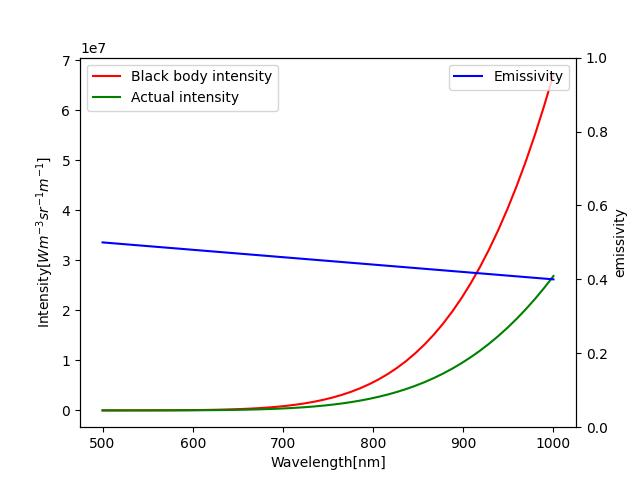
\includegraphics[width = 0.8\textwidth]{figures/real_radiation.jpg}
    \caption{Black body radiation, emissivity and real radiation of an example normal
    material at $1000K$}
    \label{fig: black_body_radiation}
\end{figure}


In Fig.\ref{fig: black_body_radiation} can be found, that the real spectral 
intensity of a normal material is lower than the black body spectral intensity.
And the emissivity of the material varies with the increase of the radiation 
wavelength.


It can be seen that the construction of a reliable emissivity model is crucial to 
the accuracy of the virtual experimental platform. It is the key component used to 
generate the experimental data.




\section{Virtual experiment platform}%
After obtaining the physical spectral intensity of the material, a virtual experiment platform
is used to transform the physical value into digital value, which simulate the 
behavior of a real spectral pyrometer. As described in Fig.\ref{fig: virtual_platform}, a 
camera with a lens system focused on the surface of the powder bed is resonsible 
for obtaining spectral radiation of the heated metal powder. It can be seen from 
Fig.\ref{fig: sensor_pixel}, each pixel of the sensor 
contains 8 filters and thus be able to obtain 8 intensity digital values in different 
channels. Thus, a virtual experiment platform with the same structure as the real 
experiment platform is built.

\begin{figure}[htbp]
    \centering
    \begin{subfigure}{0.6\textwidth}
        \centering
        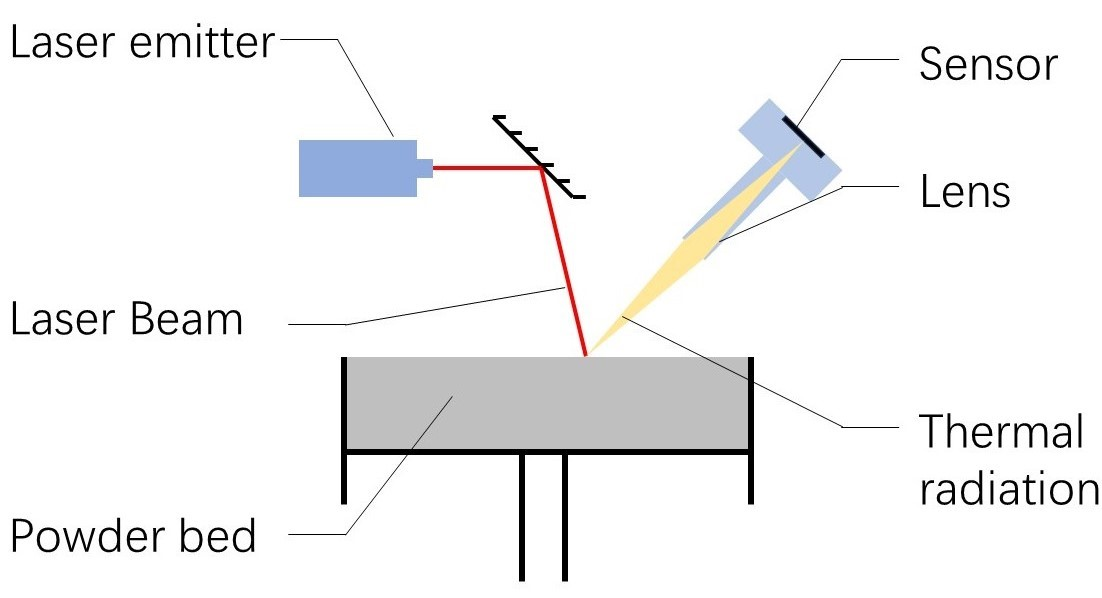
\includegraphics[height=4.8cm]{figures/virtual_platform.jpg}
        \caption{Virtual experiment platform}
        \label{fig: virtual_platform}
    \end{subfigure}
    \hfill
    \begin{subfigure}{0.37\textwidth}
        \centering
        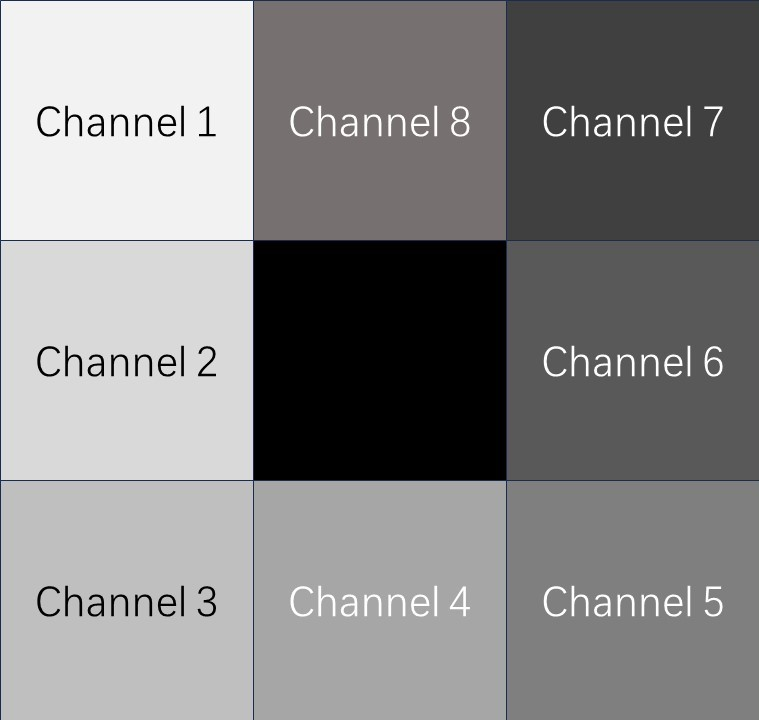
\includegraphics[height=5cm]{figures/sensor_pixel.jpg}
        \caption{Layout of a sensor pixel}
        \label{fig: sensor_pixel}
    \end{subfigure}
    \caption{Structure of the virtual experiment platform and Layout of a sensor pixel}
    \label{fig: virtual_pixel}
\end{figure}


\section{Camera model}
It can be found in Fig.\ref{fig: virtual_pixel}, The thermal radiation is emitted from the surface of powder bed, and passes through 
the lens system of the camera, finally, it reaches the sensor and be converted into 
digital values. The simplified process can be seen in Fig.\ref{fig: view_factor}. $dA_m$ is the 
area of the focused surface and $dA_{pixel}$ the area of the pixel in camera system, $n_m$ is the 
normal vector of the surface.

\begin{figure}[htbp]
    \centering
    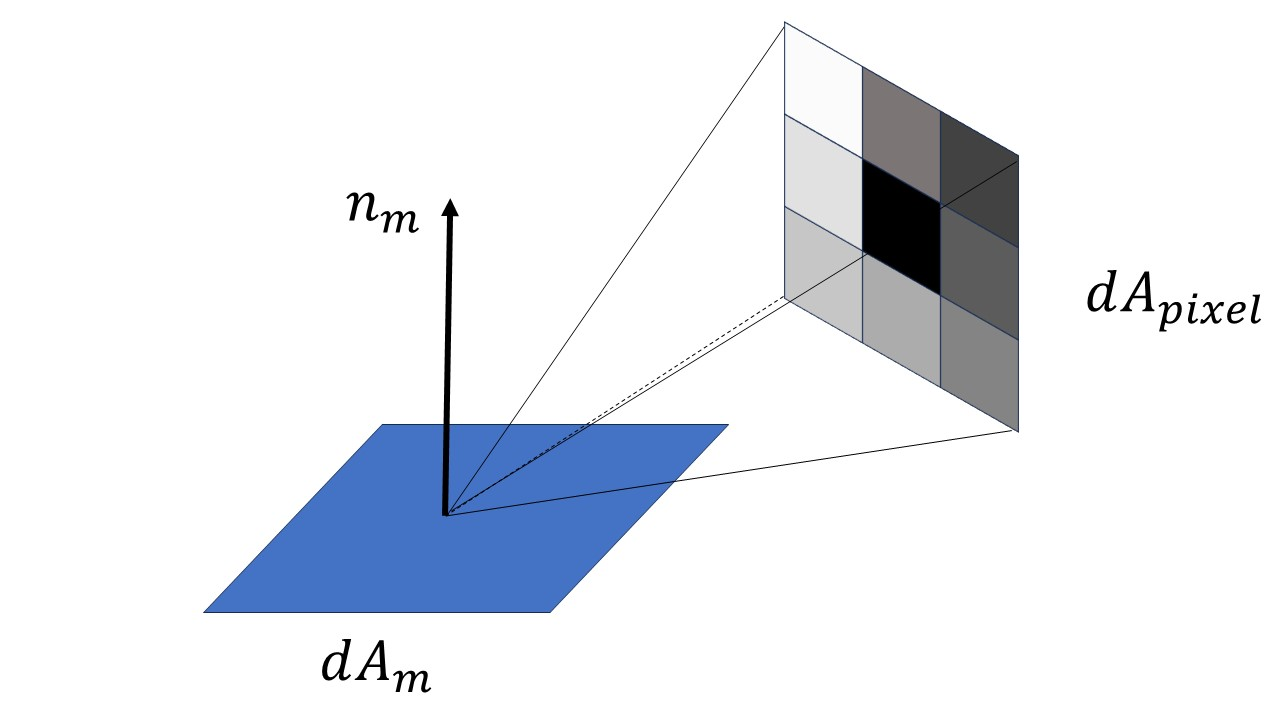
\includegraphics[width=0.6\textwidth]{figures/view_factor.jpg}
    \caption{Radiative exchange between camera system and powder bed}
    \label{fig: view_factor}
\end{figure}


\begin{comment}
Thus, the radiation intensity received by the camera system can be expressed in Eq.\ref{eq: physical_value_received}.
Where $dL_{sensor}$ means the spectral intensity reached on each channel, $dL_{material}$
is the spectral intensity emitted from the surface area, $\phi_{dA_m - dA_{pixel}}$ is the 
view factor between the focused surface area and camera system.

\begin{equation}
    \label{eq: physical_value_received}
    dL_{sensor} =  dL_{material} \cdot \phi_{dA_m - dA_{pixel}}
\end{equation}


The view factor describes the ratio between the emitted intensity of the surface area 
and the received intenisty by the pixel in camera. It only relates to the shape of 
the two surfaces and the geometric position between them\cite{Rohsenow.1998}. Since 
in real experiments, the sensor is fixed in a certain position on the machine while the 
surface of the powder bed does not move relatively to the machine, it can be concluded
that the geometry of the camera system and the focused area does not change. This means that 
the view factor does not change as the process proceeds.


So, in order to simplify the physical model of the virtual experiment platform and 
thus avoid unnecessary complexity, one assumption was made that the view factor between 
surface area of the powder bed and the camera system is constantly set to 1.
\end{comment}


\subsection{Frequency response}
After obtaining the virtual experiment platform and knowing the external setup of the 
sensor, the internal effects of the camera system should also be taken into account 
in the complete virtual experiment platform.


In order to simulate real camera system, the frequency response of sensor and lens 
should be considered. In real camera systems, all spectral radiation will 
pass through the lens system of camera. Since the lens system is not an 
idealized system, the effect of the lens system is not negligible. 

\begin{figure}[htbp]
    \centering
    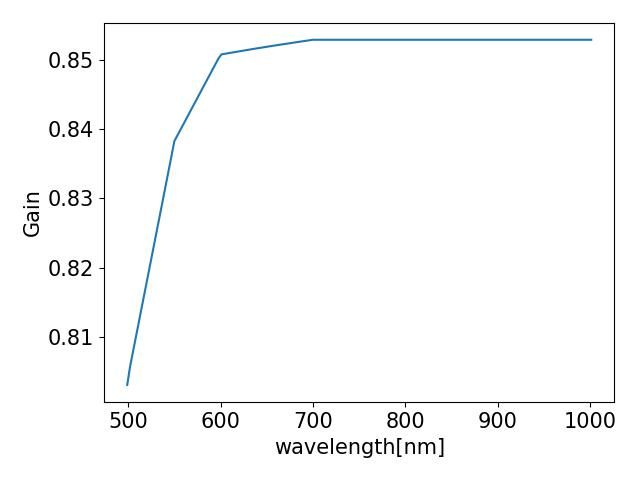
\includegraphics[width=0.6\textwidth]{figures/tr_frequency_response.jpg}
    \caption{Frequency response of the lens system}
    \label{fig: frequency_response_lens}
\end{figure}


It can be found in Fig.\ref{fig: frequency_response_lens} that system gain 
of lens system is not constant. In the wavelength range of 500 to 700 nanometers, 
the lens is more sensitive to the radiation with long wavelength. With the 
increasing wavelength, the system gain of the lens system keep constant at 0.853.


In addition to the fact that the lens system respond differently to radiation
with different wavelengths, the sensor of the camera also have wavelength-dependent quantum 
efficiency. As mentioned in previous section, the acquisition of the spectral 
intensity by the sensor for different channels is based on the filter 
before the pixels. 


Fig.\ref{fig: quantum_efficiency} shows the quantum efficiency 
of the camera sensor in different channels. Unlike an ideal sensor that 
receives only single wavelength radiation, the intensity information received 
by a real sensor is a combination of a spectral radiation and 8 filters with 
different frequency responses. Thus, the camera system is able to obtain the 
spectral radiation intensity in 8 channels simutaneously. 


\begin{figure}[htbp]
    \centering
    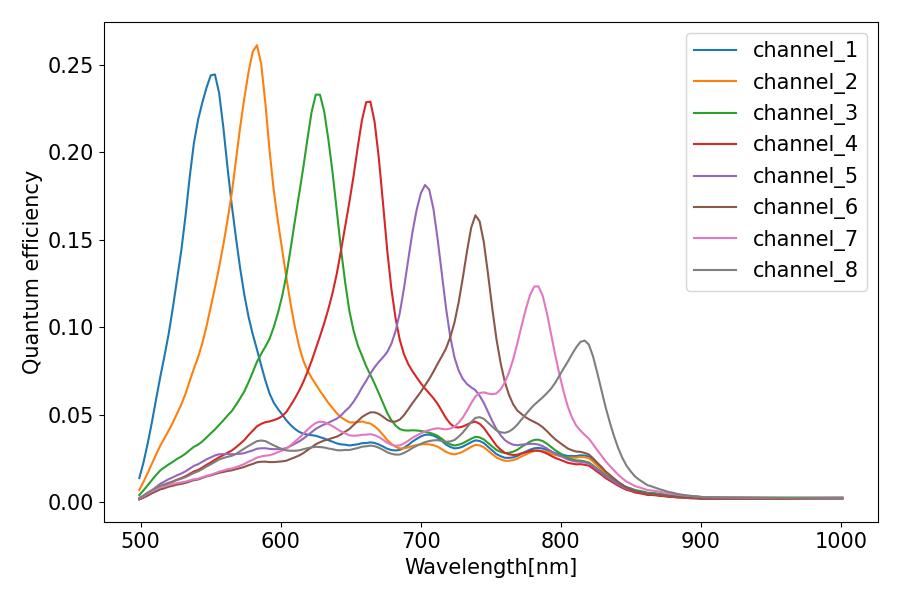
\includegraphics[width = 0.8\textwidth]{figures/quantum_efficiency.jpg}
    \caption{Quantum efficiency of camera system in each channel}
    \label{fig: quantum_efficiency}
\end{figure}


To make the virtual experiment platform more comparable to real experiments, 
it can be concluded that it is necessary to build a camera model that 
incorporates the effects of sensor quantum efficiency and lens transparency.
Then, the physical value of the spectral radiation intensity could be 
calculated accurately by the digital value of spectral radiation intensity obtained from the virtual experiment 
platform.


\subsection{Integration method}
As a result, the process of converting the physical values of radiation intensity 
into digital values needs to be accurately reproduced. Since the total efficiency 
of the camera (${\eta}_{camera}$) was delivered by quantum efficiency (${\eta}_{quantum}$)
of the sensor and transparency of the lens system{$\tau_{lens}$}, the mathematical
relationship could be described in Eq.\ref{eq: cam_efficiency}.


\begin{equation}
    \label{eq: cam_efficiency}
    {\eta}_{camera} = {\eta}_{quantum} \cdot \tau_{lens}
\end{equation}


Fig.\ref{fig: received} shows the relationship between the incoming spectral 
radiation intensity and actual captured spectral radiation intensity 
by the camera system. It can be found that the wavelength of the spectral 
radiation intensity actually received by the sensor deviates from the wavelength of the 
spectral radiation intensity it supposed to receive.


\begin{figure}[htbp]
    \centering
    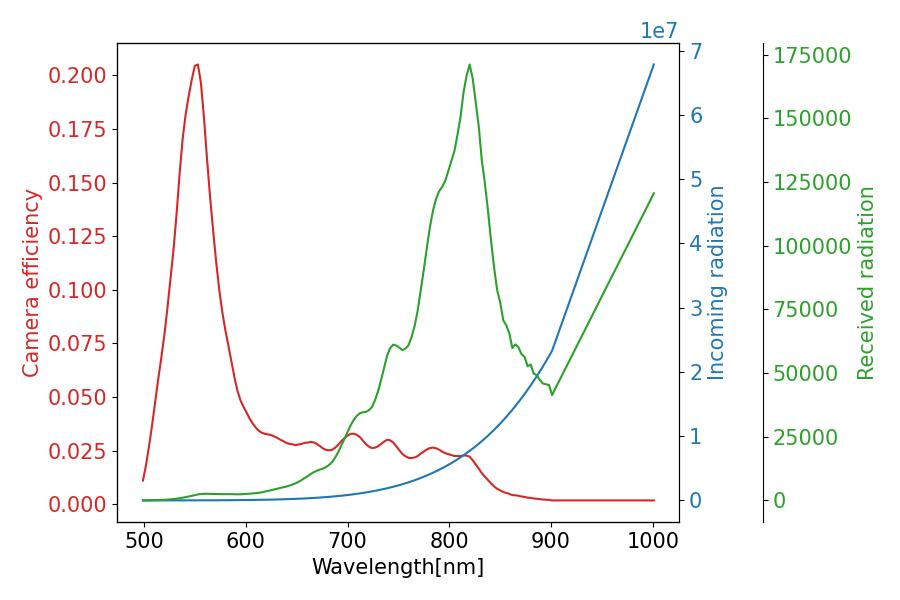
\includegraphics[width = 0.8\textwidth]{figures/received_radiation.jpg}
    \caption{Actual received spectral radiation intensity by channel 1 at 1000K}
    \label{fig: received}
\end{figure}


Obtaining the physical value of spectral radiation intensity, the sensor is responsible 
for transforming the physical value into digital value for upcoming proceedings.
The camera system used in real experiment platform uses \gls{ccd} or \gls{cmos}
as their sensors. Both sensors transform the photon flux $\phi (\lambda)$ 
incident on the semiconfuctor into photocurrent $I_{ph}$\cite{Fossum.2014}. 

\begin{equation}
    \label{eq: principle_cmos}
    I_{ph} = q \int_{\lambda}^{} \phi(\lambda) \cdot \eta_{camera}(\lambda) d\lambda
\end{equation}

With a certain temperature $T$: 

\begin{equation}
    \label{eq: quantum_flux_intensity}
    \phi(\lambda) = L(\lambda, T)
\end{equation}

Eq.\ref{eq: principle_cmos} is the mathetical description of the 
transformation. Where $\phi(\lambda)$ denotes photon flux on the sensor, 
which is equal to the spectral radiation intensity on the sensor $L(\lambda, T)$ as 
described in Eq.\ref{eq: quantum_flux_intensity}, and $\eta_{camera}(\lambda)$
denotes the total efficiency of the camera in Eq.\ref{eq: cam_efficiency}. $q$ is the sensitivity parameter 
of the sensor.


\subsection{Implementation}
Similar to the method used to obtain the digital value of spectral radiation intensity 
in the real experiment, the virtual experiment platform calculates the 
intensity digital value in 8 channels using the virtual camera by entering 
the material properties of the point being measured.


\begin{figure}[htbp]
    \centering
    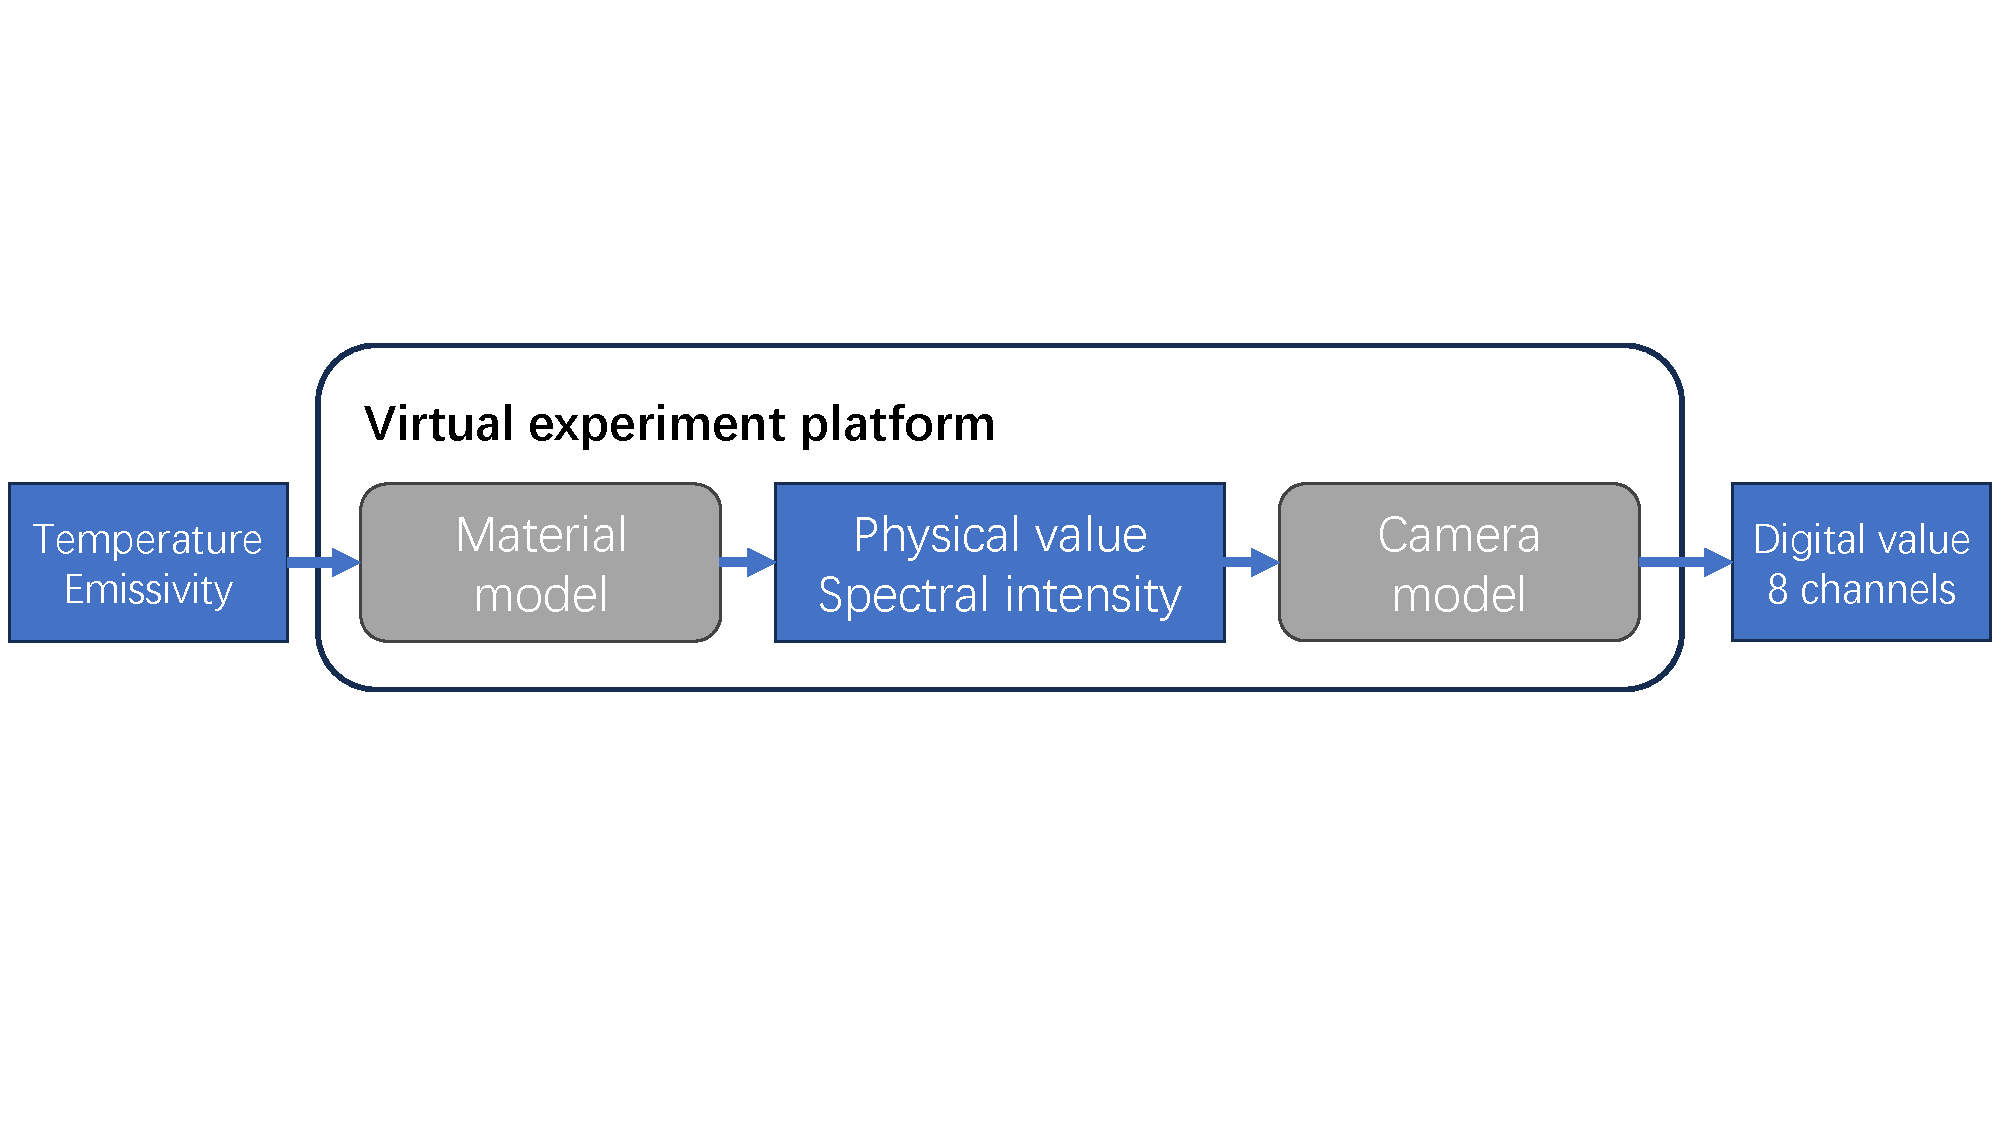
\includegraphics[width=0.95\textwidth]{figures/camera_model.pdf}
    \caption{Procedure of using virtual experiment platform to generate digital values}
    \label{fig: process_virtual_platform}
\end{figure}

Fig.\ref{fig: process_virtual_platform} shows the working procedure of the 
virtual experiment platform. 
To enable the virtual experimental platform to run on various devices, 
the entire platform has been implemented using Python as the 
programming language and packaged into a .py file. Furthermore, all 
functions have been vectorized to facilitate the generation of image 
outputs resembling those captured by a physical camera. Additionally, 
the parallel computing package in Python has been utilized to minimize 
computation time.


\section{Temperature estimation algorithm}
After obtaining the experimental data calculated by the virtual experiment platform, 
a temperature estimation algorithm should be developed to calculate the temperature 
of the measured point based on the experimental data.


Similar to the set up in real experiments, the parameters of the camera model can be 
considered as known in the virtual experimental platform mentioned in this article. 
This will on the one hand improve the accuracy of the temperature estimation algorithm
and on the other hand avoid some unnecessary complexity.


Thus, in this temperature estimation algorithm, the known variable is the digital value of 
spectral intensity captured by camera model in virtual experiment platform, the characteristic 
of the camera system. The variables to be estimated are the temperature of the measured point and 
its emissivity.


\begin{figure}[htbp]
    \centering
    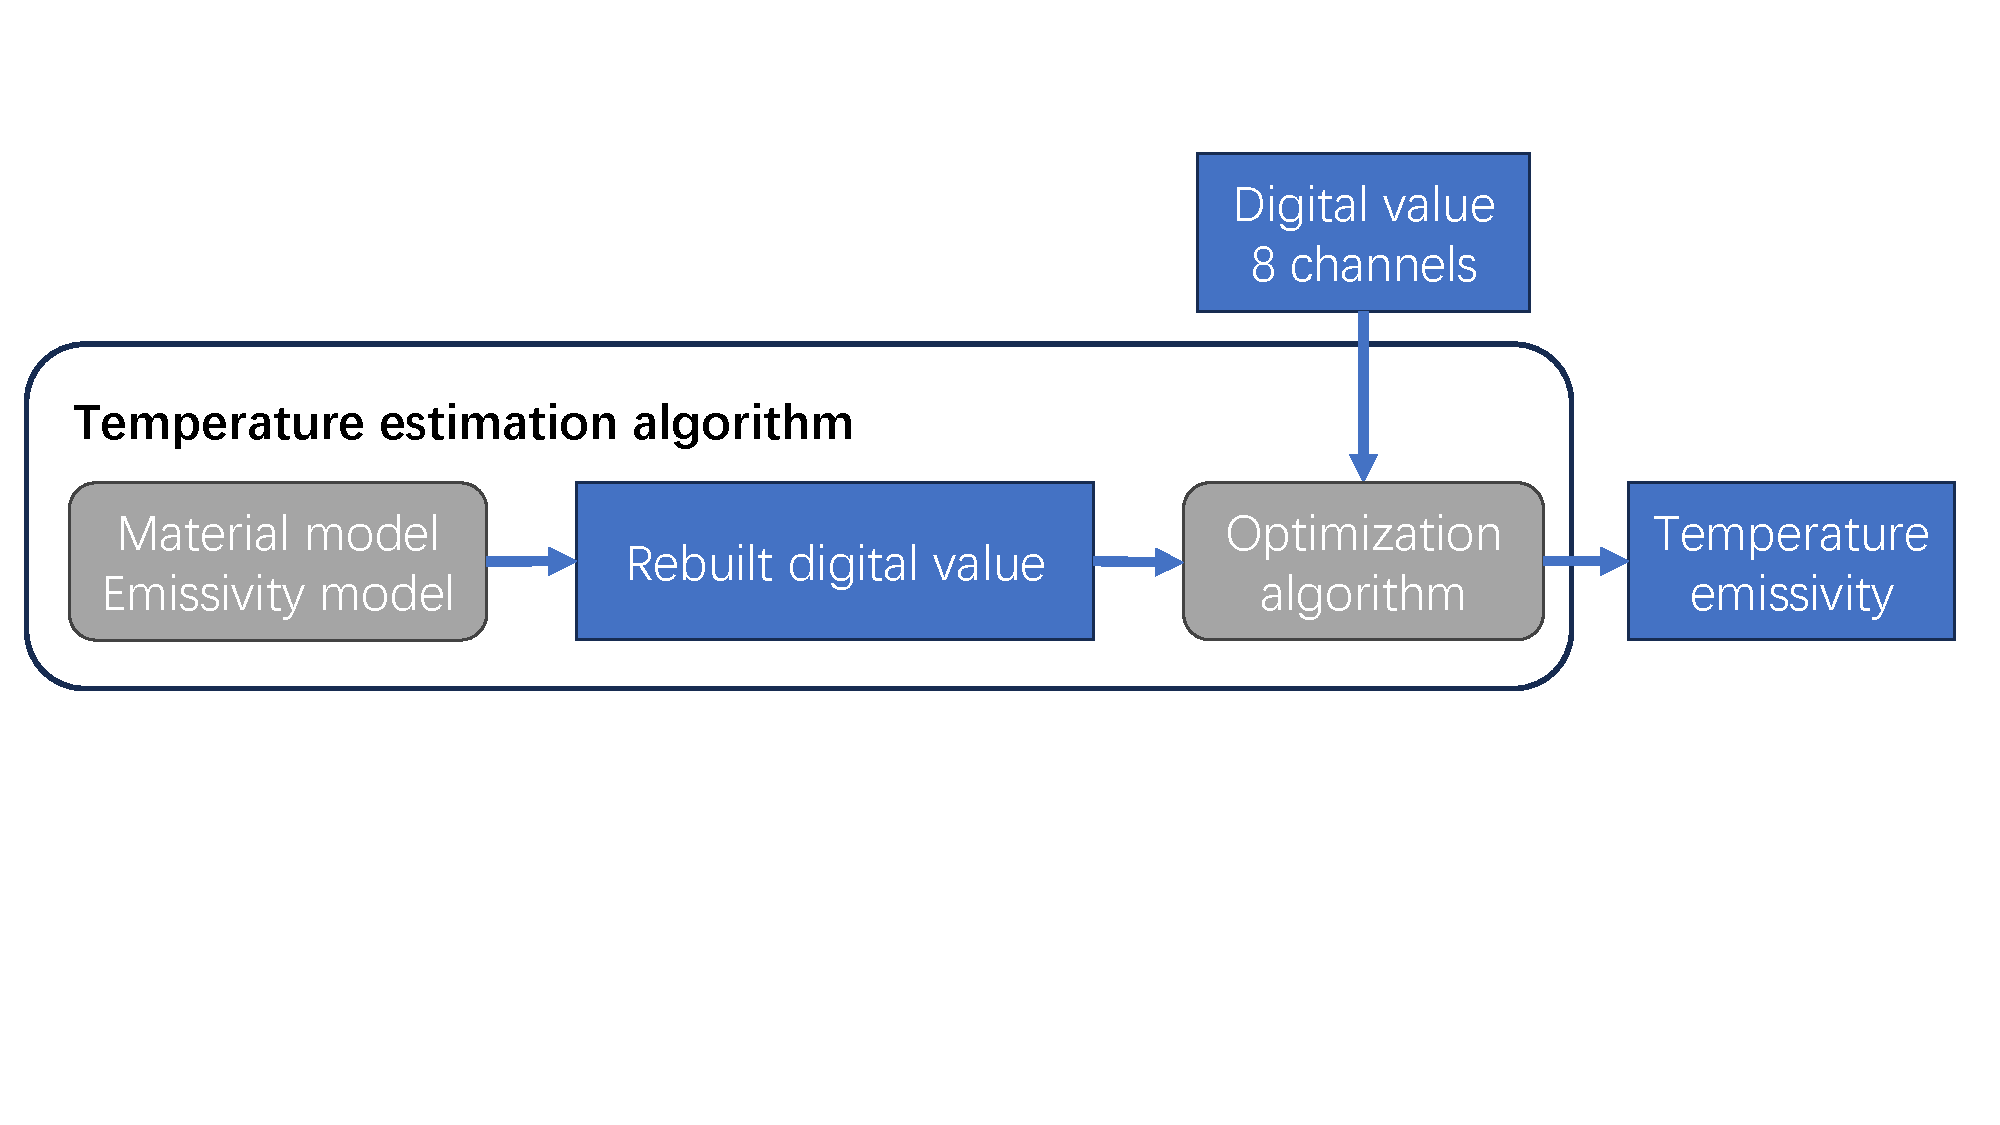
\includegraphics[width=0.95\textwidth]{figures/temperature_esti_algorithm.pdf}
    \caption{Procedure of temperature estimation algorithm}
    \label{fig: temperature_estimation_algorithm}
\end{figure}


\subsection{Temperature estimation with integration method}
Fig.\ref{fig: temperature_estimation_algorithm} shows the proceeding procedure of the 
temperature estimation algorithm. The digital value of the spectral radiation intensity
$(I_{rec}(i))$ 
in the $i_{th}$ channel should be reconstructed in Eq.\ref{eq: reconstruct_integration}:

\begin{equation}
    \label{eq: reconstruct_integration}
    I_{rec}(i) = q \int B(\lambda, T) \cdot \varepsilon(\lambda, k, T) \cdot \eta_{camera}(i) d\lambda
\end{equation}

With $I_{DV}(i)$ the reconstructed digital value in $i_{th}$ channel, $B(\lambda, T)$ the black body radiation, 
$\varepsilon(\lambda, k, T)$ the emissivity model in temperature estimation algorithm, 
$\eta_{camera}(i)$ the total camera efficiency of $i_{th}$ channel. It can be found that 
the emissivity model have an additional parameter $k$, this parameter is used for fitting 
the emissivity behavior of the measured material. More details can be found in the following 
section.


Given an initial guess of the status parameters, namely 
temperature($T_0$) and parameters in emissivity model($k_0$). Then, an curve fit 
algorithm is applied to minimize the difference between the reconstructed digital value $(I_{rec})$ 
and the actual digital value $(I_{act})$ in Eq.\ref{eq: reconstruct_optimization}.

\begin{equation}
    \label{eq: reconstruct_optimization}
    \min_{k, T}\sum_{i=1}^{8}  F(I_{rec}(i), I_{act}(i))
\end{equation} 

$F(I_{rec}(i), I_{act}(i))$ is the cost function of the curve fit algorithm. In this 
application, Non-linear least squares method is used to obtain the optimum parameters 
as Eq.\ref{eq: least_square}.

\begin{equation}
    \label{eq: least_square}
    F(I_{rec}(i), I_{act}(i)) = (I_{rec}(i) - I_{act}(i))^2
\end{equation}


After obtaining the estimated temperature ($T_{estimate}$) and the parameter ($k$) 
in the emissivity model, the data will be saved in a .xlsx file for 
potential operations.

\subsection{Temperature estimation with linear method}
To be done


\section{Emissivity model in temperature estimation algorithm}%
As an unknown quantity in the temperature estimation algorithm, the nature of emissivity 
as a function of wavelength also introduces an additional degree of freedom 
into the overall calculation process. In order to provide a more general description of 
the trend of emissivity with wavelength, an additional parameter ($k$) in the 
emissivity model used for temperature estimation has been introduced.


Due to the inherent complexity of this trend, it is often impossible to describe 
the emissivity using a single parameter. Therefore, the parameter ($k$) is normally 
represented as a vector composed of multiple variables. This approach allows for both a 
concise mathematical representation and the incorporation of more 
intricate emissivity models into the temperature estimation algorithm.


%
%
